\section*{}
\begin{frame}{}
\begin{beamercolorbox}[colsep=1.5pt,rounded=true,shadow=true]{block body example}
    \huge{Chapter 7: Channel Reciprocity for Key Transmission (CRicKET)}
\end{beamercolorbox}
\vspace{2cm}
\textbf{Publications}:\\
C. Paschou, F. Raimondo, M. Gugala, D. McEwan, J. Pope, G. Oikonomou.
    ``CRICKET: A Practical Physical Layer Key Agreement Protocol for IoT Networks.'' In 2023 IEEE International Conference of Communications (IEEE ICC 2023), pp. 1-7. IEEE, 2023.

\end{frame}

\section{Channel Reciprocity for Key Transmission (CRicKET)}

\begin{frame}{Motivation}
\framesubtitle{The four stages of physical layer key generation}
\vspace{-.26cm}
\begin{figure}
    \centering
    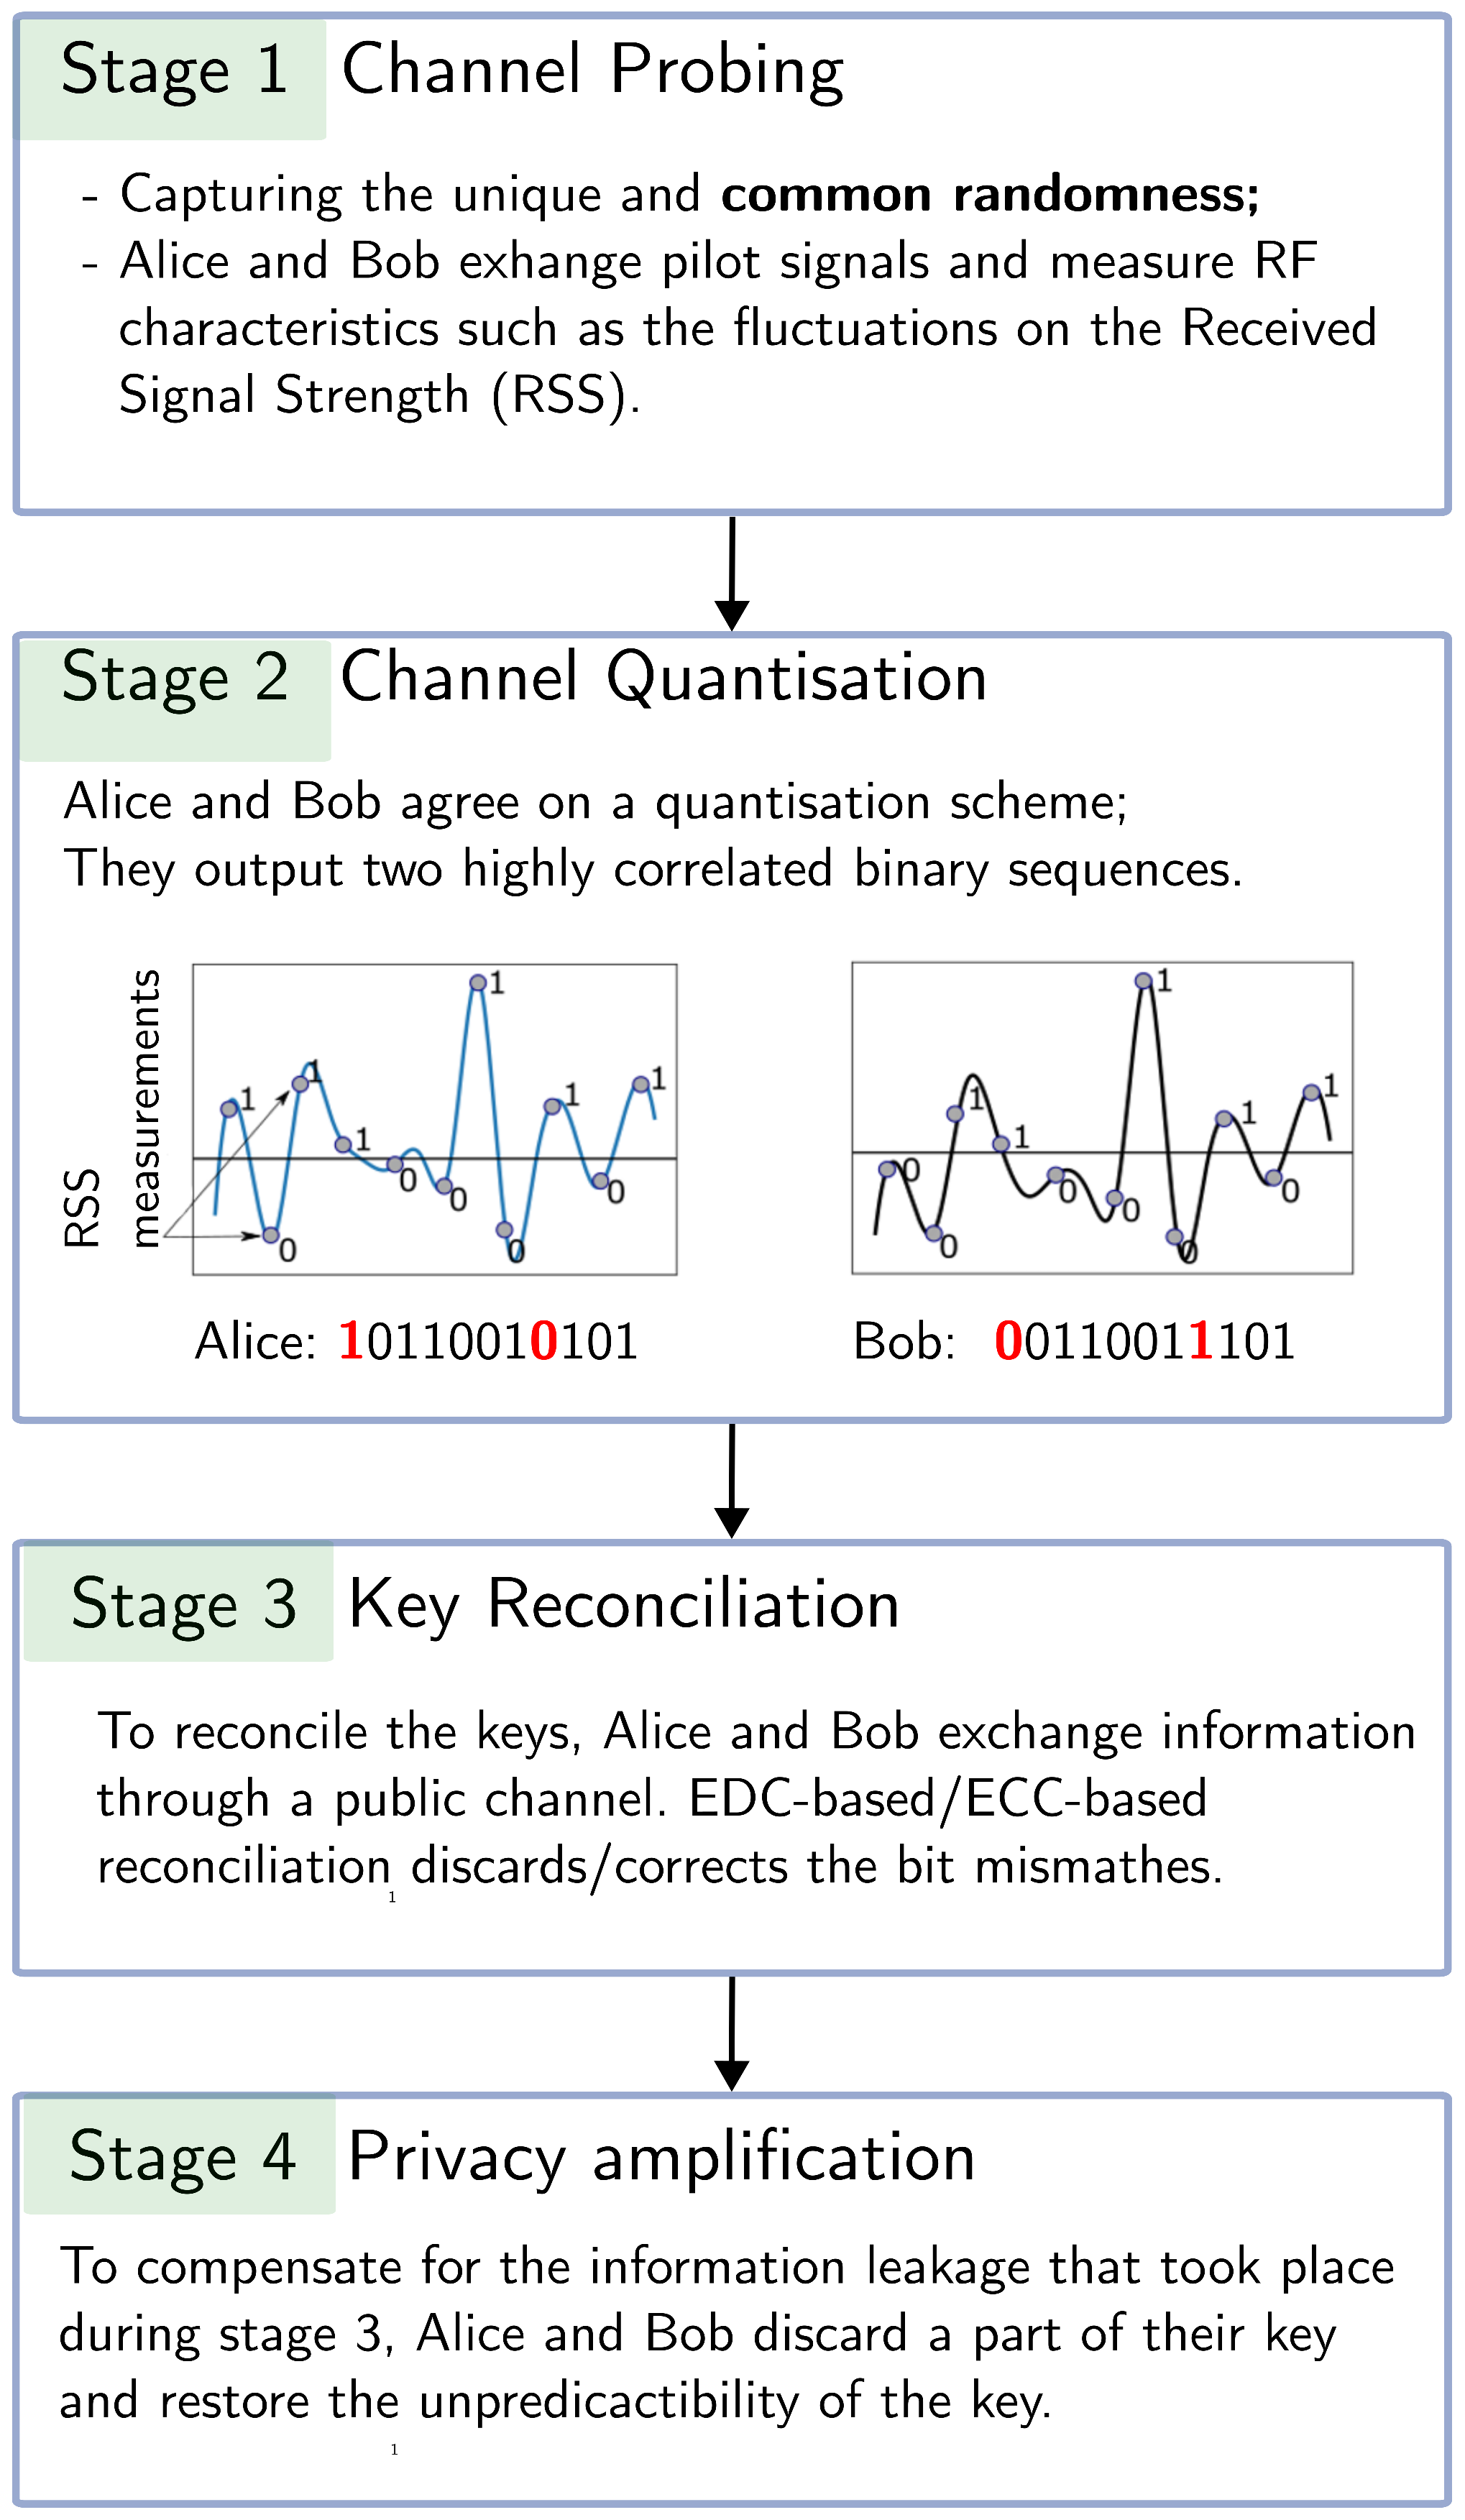
\includegraphics[scale = 0.215]{slides/figures/PLKG.eps}
    \caption{Caption}
    \label{fig:PLKG}
\end{figure}
\end{frame}

\begin{frame}{Motivation}
\framesubtitle{The four stages of physical layer key generation (cont.)}
\vspace{-.5cm}
\begin{figure}
    \centering
    \includegraphics[scale = 0.7]{slides/figures/KGR2.jpg}
    \caption{The four stages of a typical physical layer key generation protocol.}
    \label{fig:PLKG2}
\end{figure}
\end{frame}


\begin{frame}{Motivation}
\framesubtitle{Current Limitations of Physical Layer Key Generation Protocols}
\begin{itemize}
    \item With typical Physical Layer Key Generation (PLKG):\\ high key disagreement rate $\rightarrow$ high reconciliation cost;
    \item High reconciliation cost $\rightarrow$ PLKG is impractical in resource-constrained networks.    
\end{itemize}
\begin{table}
    \centering
    \begin{tabular}{|c|ccc|}
    \hline
        \textbf{Approach} & \textbf{Comm.Overhead} & \textbf{Complexity} & \textbf{Leakage} \\
        \hline
        EDC-based & High & Low & Low\\
        ECC-based & Low & High & High\\
        \hline
    \end{tabular}
    \caption{A high-level comparison between EDC-based approaches and ECC-based approaches for key reconciliation.}
\end{table}
\end{frame}

\begin{frame}{Motivation}
\framesubtitle{Solution}
\begin{itemize} 
    \item CRicKET is a coding scheme for key transfer that keeps the key disagreement rate (KDR) arbitrarily low;
    \item Arbitrarily low KDR $\rightarrow$ arbitrarily low reconciliation cost;
    
    \item A low reconciliation cost trades off on encoding rate and not on computational complexity;
    \item CRicKET is a good fit for delay-tolerant applications with low computational capabilities. 
\end{itemize}
\end{frame}

\begin{frame}{CRicKET}
\begin{figure}
    \centering
    \vspace{-1.25cm}
    \includegraphics[scale = 0.4]{figures/Cricket/cricket vs PLKGv2.pdf}
    \caption{PLKG vs CRicKET}
    \label{fig:enter-label}
\end{figure}    
\end{frame}

\begin{frame}{Tunable parameters}
\begin{block}{Notation and Terminology}
\begin{beamercolorbox}[rounded=true]{block body}\textbf{Channel sequence}: the sequence obtained during the channel probing phase; \\
\textbf{Channel mismatch} ($p_{\text{ch}}$): measure of the difference between the channel sequence at Bob and the channel sequence at Alice;\\
$\mathbf{n}$, $\mathbf{\tau}$: coding parameters.
\end{beamercolorbox}
\end{block}

\begin{table}
    \centering
    \begin{tabular}{|c||ccccccccc|}
        \hline
       $p_{\text{ch}}$  & 0.05 & 0.1& 0.15&0.2 &0.25&0.3 &0.35&0.4 &0.45\\
        \hline
         \hline
       $n$ & 3& 5& 4 & 10& 15& 19& 28 &35& 54\\
        \hline
       $\tau$ & 0 & 0 & 0& 3 & 5& 6& 9& 9& 9 \\
        \hline
    \end{tabular}
    \caption{Optimal parameters for different values of $p_{\text{ch}}$ when the system's requirement is KDR < 0.001.}
    \label{tab: optimal}
\end{table}
\end{frame}

\begin{frame}{Encoding Rate vs Channel Miss-match}
\framesubtitle{}

\begin{figure}
    \centering
    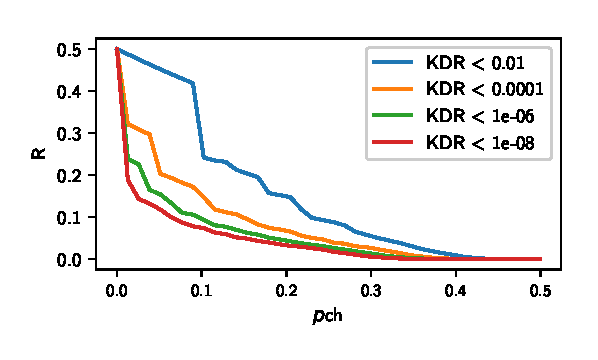
\includegraphics[scale = 0.9]{figures/Cricket/optimal_param.eps}
    \caption{Achievable encoding rates against channel mismatch for different requirements for the key disagreement rate.}
    \label{fig:acheivable rates}
    \end{figure}
\end{frame}

\begin{frame}{Implementation}
\begin{figure}
    \centering
    \includegraphics[scale = 0.9]{figures/Cricket/devices2.pdf}
    \caption{Caption}
    \label{fig:enter-label}
\end{figure}
    
\end{frame}

\begin{frame}{Implementation}
\begin{figure}
    \centering
    \includegraphics[scale = 0.5]{figures/Cricket/cricket_implentation.pdf}
    \caption{Flow diagram.}
    \label{fig:enter-label}
\end{figure}
\end{frame}

\begin{frame}{Implementation}
\framesubtitle{Experimental Results}
\begin{figure}
    \centering
    \includegraphics[scale = 1.2]{figures/Cricket/boxplots.pdf}
    \caption{Caption}
    \label{fig:enter-label}
\end{figure}
\end{frame}

\begin{frame}{Information Theoretic Guarantees}

\begin{itemize}
    \item CRicKET is proven to achieve perfect secrecy even when the channel sequences have low entropy \footnote{Under the assumption of decorrelated fading. I.e., Eve is assumed to be sufficiently distanced from the legitimate receivers.};
    \item By combining CRicKET with a high-level quantisation scheme or a ``smoothening'' filtering mechanism, it is possible to increase the key rate and decrease the vulnerability to brute-force attacks.
\end{itemize}
\end{frame}

\begin{frame}{Concluding Remarks}
\begin{itemize}
    \item {CRicKET} is a key agreement protocol designed for low-cost devices due to its minimal computational complexity and low memory requirements.

\item The parameters of {CRicKET} can be configured to achieve a desired key disagreement rate, and its analytical results have been validated.
\item A practical implementation over a low-rate wireless personal area network has demonstrated its suitability for IoT devices.
\end{itemize}
    
\end{frame}